\documentclass{article}
\usepackage{amsfonts}          % Para las negrita de pizarra
\usepackage{indentfirst}       % Para que quede mas lindo el formateo
\usepackage{graphicx}          % Para graficos
\usepackage{minted}            % Para poner codigo y que quede con sintaxis fachera
\usepackage{hyperref}          % Para meter hipervinculos
\usepackage[dvipsnames]{xcolor}% Para usar colores
\usepackage{hhline}            % Mas configuracion para las lineas en tablas
\usepackage{amsmath}           % Agregado para tags de ecuaciones
\usepackage{xcolor}            % Coloreado de ecuaciones
\usepackage{quoting, xparse}   % Usado para citar
% \usepackage{svg}               % Para usar imagenes svg que se ven lindas independientemente del zoom. WARNING REQUIERE DE INKSCAPE. Tal vez no vale la pena
\usepackage{amsmath}

\graphicspath{ {./images/} }

\newcommand{\docuPy}{%
  {\href{https://wiki.python.org/moin/TimeComplexity}{documentacion oficial}}
  }%

  % Comandos para facilitar el citado
  % Fuente: https://tex.stackexchange.com/a/391739/273865
\NewDocumentCommand{\bywhom}{m}{% the Bourbaki trick
  {\nobreak\hfill\penalty50\hskip1em\null\nobreak
   \hfill\mbox{\normalfont(#1)}%
   \parfillskip=0pt \finalhyphendemerits=0 \par}%
}

% Esta funcion en realidad es una mentira. Emula ser una funcion de latex. La idea
% es que el makefile que corre esto vea la funcion y la reemplace correctamente
% 
\newcommand{\funcionArchivo}[2]{%
  {\textcolor{red}{WARNING: SI ESTAS VIENDO EN EL PDF SIGNIFICA QUE ALGO ANDUVO MAL. ASEGURATE DE COMPILAR EL LATEX CON EL MAKEFILE. GRACIAS :D}}
  }%

\begin{document}

\begin{titlepage}
  \vspace*{1cm}

  \begin{center}
    {\Huge{Trabajo Práctico 2: Programación Dinámica para el Reino de la Tierra}}
  \end{center}

  \vspace{0.4cm}

  \begin{center}
    {\LARGE{Facultad de Ingeniería de la Universidad de Buenos Aires}}\\
    \vspace{0.3cm}
    {\Large{Teoría de Algoritmos}}\\
    \vspace{0.3cm}
    {\large{Cátedra Buchwald-Genender}}\\
  \end{center}

  \vspace{0.8cm}
  \begin{center}
    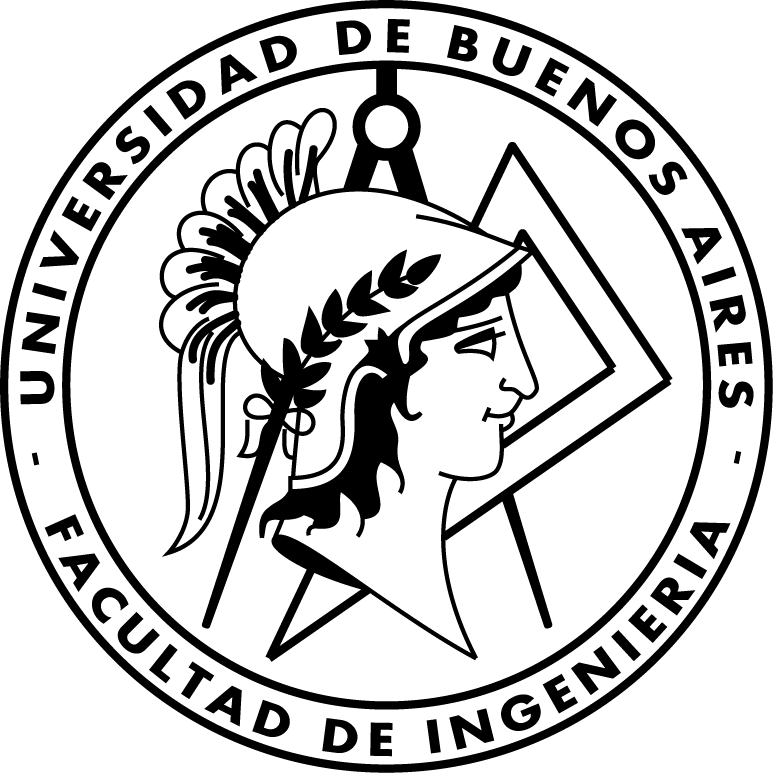
\includegraphics[scale=0.8]{Logo-fiuba}
  \end{center}

  \vspace{1.4cm}
  \begin{center}

    {\begin{minipage}[t]{.32\textwidth}
        \begin{center}
          Gómez Belis, Sofía\\
          {\small{Padrón: 109358}}\\
          {\small{email: sgomezb@fi.uba.ar}}
        \end{center}
          \end{minipage}
          \begin{minipage}[t]{.32\textwidth}
        \begin{center}
          Llanos Pontaut, Valentina\\
          {\small{Padrón: 104413}}\\
          {\small{email: vllanos@fi.uba.ar}}\\
        \end{center}
      \end{minipage}
      \begin{minipage}[t]{.32\textwidth}
        \begin{center}
          Orsi, Tomas Fabrizio\\
          {\small{Padrón: 109735}}\\
          {\small{email: torsi@fi.uba.ar}}
        \end{center}
      \end{minipage}}

  \end{center}
\end{titlepage}

\renewcommand*\contentsname{Indice}
\tableofcontents
\pagebreak

\section{Análisis del problema}
\subsection{Descripción y objetivo}
TO-DO
\subsection{Análisis y ecuación de recurrencia}

La resolución de un problema por medio de la programación dinámica implica reutilizar las soluciones a subproblemas más pequeños en problemas más grandes que los incluyan. En el contexto actual, el foco está puesto en maximizar la cantidad de enemigos eliminados dados \texttt{n} minutos. Esta variable \texttt{n} es crucial en el análisis del problema planteado puesto que si se tiene \texttt{k} minutos, con $k < n$, necesariamente la solución será menor o igual (solo son iguales si no llegan enemigos en el minuto \texttt{n} y $n = k - 1$) a la solución en el minuto \texttt{n}. De esta forma, la cantidad de minutos que tiene el ataque repercute en el resultado final del combate. Por ejemplo, si $n = 0$, se puede afirmar que la cantidad de enemigos eliminados será también 0. Entonces, nuestros subproblemas estarán dados por la cantidad máxima de enemigos que se pueden eliminar en cada minuto $i \leq n$.

Sabiendo la forma de los subproblema, debemos analizar cómo se componen para resolver subproblemas más grandes. Si queremos obtener la solución óptima en el minuto \texttt{i}, vamos a poder utilizar las soluciones parciales calculadas hasta entonces, pero no nos interesa si existen o no problemas más grandes. Si estamos en el minuto $i = n$, sabiendo que es el último, tenemos dos estrategias posibles: atacar o cargar. ¿Tiene sentido cargar sabiendo que no se puede atacar a más enemigos? No. Esto se debe a que la cantidad de enemigos que se podrá eliminar en ese minuto será  mayor o igual a 0, pero si cargamos energía, será definitivamente nula. Por lo tanto, en el último minuto conviene siempre atacar. Ahora bien, como establecimos antes, en el minuto $i \leq n$ no importa si $i = n$ o $i < n$, solamente debemos calcular el óptimo actual. En base al análisis previamente presentado, siempre va a ser mejor atacar a cargar, más allá de que en la solución final (problema mayor) se lleve a cabo la estrategia opuesta debido a que eso esté contemplado en el óptimo del minuto n. 

Si en el minuto \texttt{i} los Dai Li atacan, la cantidad de enemigos eliminados en ese instante será $min(f(j), x_i)$. El valor de $x_i$ es conocido, pero la energía acumulada por la policía secreta de la ciudad depende de los minutos que pasaron desde el último ataque. De esta manera, tenemos una segunda variable involucrada en el problema: \texttt{j}. Si el último ataque fue realizado hace un minuto, actualmente se podrá eliminar $min(f(1), x_i)$ enemigos y la cantidad máxima acumulada será la suma entre este valor y el correspondiente valor en el ataque anterior. ¿Qué sucede si el óptimo hace dos minutos es mayor que en el minuto anterior o su suma con $min(f(2), x_i)$ lo es? Como queremos maximizar el resultado final, claramente nos conviene haber atacado hace dos minutos, lo cual también indica que en el minuto $i - 1$ se cargó energía. Tenemos varias opciones para el ataque anterior, más precisamente $1 \leq j \leq i$, pero utilizaremos aquel que nos lleve a la mejor solución. Entonces, el óptimo para el minuto \texttt{i} será la suma entre $min(f(j), x_i)$ y el óptimo en el minuto $i - j$.

Sabiendo la forma de los subproblemas y la manera en que éstos se combinan, podemos plantear la ecuación de recurrencia para el minuto \texttt{i}:

$
opt[i] = max(min(f(j), x_i) + opt[i - j]) \forall j \in [1; i]
$

Como caso base, tenemos que en el minuto 0 se eliminan 0 enemigos.

Encontrada la ecuación de recurrencia, procedemos a aplicarla iterativamente de manera bottom up, construyendo las soluciones a los subproblemas de $i < n$ hasta llegar a la solución del problema original con $i = n$. Esta técnica es justamente programación dinámica. Empleamos \texttt{memoization} guardando los resultados calculados previamente en un arreglo. El procedimiento explicado nos permite realizar una exploración implícita del espacio de soluciones. La solución final será óptima porque en el minuto \texttt{n} elegimos haber atacado hace \texttt{j} minutos, donde \texttt{j} maximiza la ecuación de recurrencia.

\section{Complejidad algorítmica}
\subsection{Complejidad lectura de archivos}
Antes de comenzar el algoritmo, tenemos que generar las listas de elementos sobre las cuales éste va a operar.
Para esto tenemos la siguiente porción de código:
\funcionArchivo{codigo/archivos.py generarTestDe}

La función lee la linea que contiene la cantidad de valores que van a tener ambas listas. Una vez hecho eso, lee $n$ lineas para almacenar los distintos valores de $x_i$ y luego lee otras $n$ lineas para tener los valores de $f(i)$.

\subsection{Complejidad algoritmo}
\funcionArchivo{codigo/algoritmo.py eliminar_enemigos}
El algoritmo empieza creando una lista de tamaño $n + 1$; lo cual, según la \docuPy, lleva $\mathcal{O}(n)$ ya que se realiza $n$ veces una operación de tiempo $\mathcal{O}(1)$.

Luego, en la linea \texttt{7} comienza un ciclo for que recorre todos los valores de $n$; todo este ciclo tiene una complejidad $\mathcal{O}(n)$.

Luego en la linea \texttt{9} comienza un nuevo ciclo for, el cual va desde 0 hasta el valor actual de $n$. Esto significa que, en el peor de los casos, este ciclo va a iterar hasta $n$. Dentro del ciclo, todas las operaciones son $\mathcal{O}(1)$.

Esto significa que la complejidad algorítmica de las lineas \texttt{7} a \texttt{17} es $\mathcal{O}(n^2)$.

Luego, en la linea \texttt{20} se ejecuta la funcion \texttt{obtener\_secuencia\_estrategias}, la cual analizamos en \nameref{sec:reconstruccion}.

Finalmente, en la linea \texttt{21} se ejecuta el método \texttt{reverse()}, el cual tiene complejidad $\mathcal{O}(n)$

Es decir que el algoritmo dinámico tiene una complejidad $\mathcal{O}(n^2)$.

\subsection{Complejidad reconstrucción}
\label{sec:reconstruccion}

\funcionArchivo{codigo/algoritmo.py obtener_secuencia_estrategias}
La reconstrucción de la secuencia estratégica empieza desde el ultimo minuto, hasta 0.
Vemos que en la linea \texttt{26} comienza un ciclo while, el cual tiene dentro un ciclo for.
Dentro del for todas las operaciones son de complejidad $\mathcal{O}(1)$, siendo todas simples operaciones.

En el peor de los casos, podemos pensar a estos dos ciclos como dos ciclos for que iteran desde 0 hasta $\texttt{n}$.(esto va a suceder en la primera iteración del algoritmo). Por esto, decimos que la reconstrucción va a tener una complejidad de $\mathcal{O}(n^2)$.

\subsection{Efecto de las variables sobre el algoritmos}

\section{Mediciones de tiempo}
\label{sec:medTiempo}
Para corroborar la complejidad algorítmica de nuestra implementación, realizamos una serie de tests de volumen. A diferencia del \href{https://github.com/La-sociedad-del-silencio/TP1-Greedy}{TP1} y debido a la complejidad temporal del algoritmo; realizamos tests con una menor cantidad de casos.
Realizamos al rededor de ~3500 tests, con $n$ entre 1 y 10000, para poder graficar y analizar el comportamiento de la implementación. El código que usamos para generar los tests se encuentran en el archivo \texttt{codigo/grafico\_complejidad.py}.

Obtuvimos los siguientes resultados:

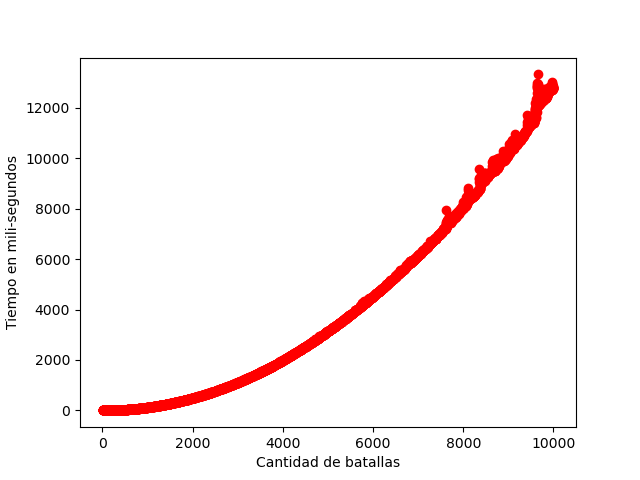
\includegraphics[scale=0.69]{miliSegsFuncCantidadNativo.png}

Observando el gráfico podemos entender mejor el comportamiento de nuestra implementación.

Podemos ver que el gráfico tiene una forma cuasi parabolica, lo cual refleja el comportamiento cuadratico del algoritmo.

Además, podemos ver el rápido crecimiento que toman los valores. Por ejemplo, 2000 batallas tardan alrededor de ~500 milisegundos y que con 4000 batallas el algoritmo tarda alrededor de ~2000 milisegundos. Vemos que al duplicar el tamaño de la entrada, el tiempo que tarda no se duplica; sino que se cuadruplica.

Con esto concluimos que a medida que aumenta el tamaño de entrada n (cantidad de batallas), el tiempo de ejecución del algoritmo crece a un ritmo cuadrático. Ésto coincide con el análisis de complejidad previamente presentado, indicando un costo proporcional a $n^2$.





\end{document}
